\documentclass[a4paper]{scrartcl}
\usepackage[cm]{fullpage}
\usepackage{amsmath, amssymb, esint}
\usepackage{siunitx}

\usepackage{tikz, pgfplots}
\pgfplotsset{
    compat = 1.12,
    plot-scatter/.style = {
        only marks,
        error bars/.cd,
        x dir = both, y dir = both,
        x explicit, y explicit
    }
}

\begin{document}

\title{PHYS3117: YAG Laser}
\author{Donny Yang \\ z3470068}
\date{2017-09-01}
\maketitle

\section{Materials and Methods}
Please refer to the student notes of the experiment.

\section{Results}
\subsection{Injection Diode Laser Characterisation}
\begin{figure}
    \centering
    \begin{tikzpicture}
        \begin{axis}[
            xlabel = Current (\si{\ampere}),
            ylabel = Power (\si{\watt}),
        ]
            \addplot +[plot-scatter] table [
                skip first n = 11
            ] {4.1};
            \addplot [no marks, red, domain = 0:0.680115] {-0.000655758 + 0.00917582 * x};
            \addplot [no marks, black, domain = 0:0.680115] {-0.000655758 + 0.00917582 * x - 2.26216 * sqrt(5.24467e-6 - 0.0000200528 * x + 0.0000319992 * x^2)};
            \addplot [no marks, black, domain = 0:0.680115] {-0.000655758 + 0.00917582 * x + 2.26216 * sqrt(5.24467e-6 - 0.0000200528 * x + 0.0000319992 * x^2)};
            \addplot [no marks, red, domain = 0.680115:2.2] {-0.847073 + 1.2537 * x};
            \addplot [no marks, black, domain = 0.680115:2.2] {-0.847073 + 1.2537 * x - 2.26216 * sqrt(0.0000141109 - 0.000021951 * x + 9.78709e-6 * x^2)};
            \addplot [no marks, black, domain = 0.680115:2.2] {-0.847073 + 1.2537 * x + 2.26216 * sqrt(0.0000141109 - 0.000021951 * x + 9.78709e-6 * x^2)};
        \end{axis}
    \end{tikzpicture}
    \caption{Output power of the injection laser against input current, with bilinear fit and \SI{95}{\percent} CI}
    \label{fig:4.1}
\end{figure}
\begin{figure}
    \centering
    \begin{tikzpicture}
        \begin{axis}[
            xlabel = Wavelength (\si{\nano\metre}),
            ylabel = Counts (a.u.),
            width = 15cm,
            height = 10cm,
            restrict x to domain = 720:860
        ]
            \addplot +[thin, no marks, legend = 0.20] table [
                skip first n = 17,
                comment chars = >
            ] {spectra/0.20A.txt};
            \addlegendentry{\SI{0.20}{\ampere}};
            \addplot +[thin, no marks] table [
                skip first n = 17,
                comment chars = >
            ] {spectra/0.40A.txt};
            \addlegendentry{\SI{0.40}{\ampere}};
            \addplot +[thin, no marks] table [
                skip first n = 17,
                comment chars = >
            ] {spectra/0.60A.txt};
            \addlegendentry{\SI{0.60}{\ampere}};
        \end{axis}
    \end{tikzpicture}
    \caption{Spectra of the diode laser at low input currents}
    \label{fig:4.1-spectrum-low}
\end{figure}
\begin{figure}
    \centering
    \begin{tikzpicture}
        \begin{axis}[
            xlabel = Wavelength (\si{\nano\metre}),
            ylabel = Counts (a.u.),
            width = 15cm,
            height = 10cm,
            restrict x to domain = 800:810
        ]
            \addplot +[thin] table [
                skip first n = 17,
                comment chars = >
            ] {spectra/0.80A.txt};
            \addlegendentry{\SI{0.80}{\ampere}};
            \addplot +[thin] table [
                skip first n = 17,
                comment chars = >
            ] {spectra/1.00A.txt};
            \addlegendentry{\SI{1.00}{\ampere}};
            \addplot +[thin] table [
                skip first n = 17,
                comment chars = >
            ] {spectra/1.20A.txt};
            \addlegendentry{\SI{1.20}{\ampere}};
            \addplot +[thin] table [
                skip first n = 17,
                comment chars = >
            ] {spectra/1.40A.txt};
            \addlegendentry{\SI{1.40}{\ampere}};
        \end{axis}
    \end{tikzpicture}
    \caption{Spectra of the diode laser at high input currents}
    \label{fig:4.1-spectrum-high}
\end{figure}

The power measurements (with no observed dark reading) can be seen in Figure \ref{fig:4.1}. A bilinear fit was also performed, producing slopes of \SI{0.009 \pm 0.040}{\watt\per\ampere} before the knee and \SI{1.254 \pm 0.022}{\watt\per\ampere} after the knee, with a knee (or threshold) current of \SI{0.680 \pm 0.018}{\ampere}.

The spectra was taken of the laser in steps of \SI{0.20}{\ampere} up to \SI{1.20}{\ampere}, with the results shown in Figures \ref{fig:4.1-spectrum-low} and \ref{fig:4.1-spectrum-high}. Each measurement was done with a different spectrometer setting, to account for the large dynamic range (though all results were averaged over 50 readings):
\begin{itemize}
    \item \SI{0.20}{\ampere}: \SI{25}{\milli\second} integration time; Approx \SI{9}{\centi\metre} from laser
    \item \SI{0.40}{\ampere}: \SI{5}{\milli\second} integration time; Approx \SI{9}{\centi\metre} from laser
    \item \SI{0.60}{\ampere}: \SI{5}{\milli\second} integration time; ND1 Filter; Approx \SI{12}{\centi\metre} from laser
    \item \SI{0.80}{\ampere}: \SI{1}{\milli\second} integration time; ND2 + ND1 Filter; Approx \SI{15}{\centi\metre} from laser
    \item \SI{1.00}{\ampere}: \SI{1}{\milli\second} integration time; ND4 Filter; Approx \SI{25}{\centi\metre} from laser
    \item \SI{1.20}{\ampere}: \SI{1}{\milli\second} integration time; ND4 Filter; Approx \SI{25}{\centi\metre} from laser
    \item \SI{1.40}{\ampere}: \SI{5}{\milli\second} integration time; ND4 + ND1 Filter; Approx \SI{25}{\centi\metre} from laser
\end{itemize}

All of the readings in \ref{fig:4.1-spectrum-low} (\SI{0.20}{\ampere} to \SI{0.60}{\ampere}) are before the threshold current discovered above, and one can clearly see wide linewidths in the spectra. Meanwhile, all the readings in \ref{fig:4.1-spectrum-high} (\SI{0.80}{\ampere} and above) are past the threshold current, and the linewidths approach the resolution of the spectrometer.

\subsection{Transmission of the YAG crystal}
\begin{figure}
    \centering
    \begin{tikzpicture}
        \begin{axis}[
            xlabel = Wavelength (\si{\nano\metre}),
            ylabel = Counts (a.u.),
            width = 15cm,
            height = 10cm
        ]
            \addplot +[thin, no marks] table [
                skip first n = 17,
                comment chars = >
            ] {spectra/lamp.txt};
            \addlegendentry{Lamp only}
            \addplot +[thin, no marks] table [
                skip first n = 17,
                comment chars = >
            ] {spectra/lamp-with-yag.txt};
            \addlegendentry{Lamp + YAG}
        \end{axis}
    \end{tikzpicture}
    \caption{Spectra of the lamp, and lamp + YAG}
    \label{fig:4.2-spectrum-raw}
\end{figure}
\begin{figure}
    \centering
    \begin{tikzpicture}
        \begin{axis}[
            xlabel = Wavelength (\si{\nano\metre}),
            ylabel = Absorption Ratio,
            width = 15cm,
            height = 10cm,
            ymin = 0
        ]
            \addplot +[thin, no marks] table [
                skip first n = 17,
                comment chars = >
            ] {spectra/lamp-with-yag-absorption.txt};
            \addlegendentry{YAG Absorption}
        \end{axis}
    \end{tikzpicture}
    \caption{Corresponding absorption spectrum of Figure \ref{fig:4.2-spectrum-raw}}
    \label{fig:4.2-spectrum-absorption}
\end{figure}
\begin{figure}
    \centering
    \begin{tikzpicture}
        \begin{axis}[
            xlabel = Wavelength (\si{\nano\metre}),
            ylabel = Counts/Absorption (a.u.),
            width = 15cm,
            height = 10cm,
            restrict x to domain = 795:815
        ]
            \addplot +[thin] table [
                skip first n = 17,
                comment chars = >,
                y expr = {\thisrowno{1} / 5e4}
            ] {spectra/1.40A.txt};
            \addlegendentry{Laser Diode Spectrum};
            \addplot +[thin, red] table [
                skip first n = 17,
                comment chars = >
            ] {spectra/lamp-with-yag-absorption.txt};
            \addlegendentry{YAG Absorption}
        \end{axis}
    \end{tikzpicture}
    \caption{Zoomed in absorption spectrum overlaid on the diode laser's \SI{1.40}{\ampere} spectrum}
    \label{fig:4.2-overlay}
\end{figure}

The spectra measurements of both the lamp itself, and the lamp light passed through the YAG crystal are shown in Figure \ref{fig:4.2-spectrum-raw}. This was done with a \SI{20}{\milli\second} integration time, averaged over 50 readings.

The corresponding absorption spectrum is plotted in Figure \ref{fig:4.2-spectrum-absorption}, with the highest absorption peak at \SI{808.8 \pm 0.2}{\nano\metre}. There is also a peak at \SI{805.3 \pm 0.2}{\nano\metre}, and when combined with the highest absorption peak, are the peaks closest to the laser diode's emission wavelength of \SI{805}{\nano\metre}, as shown in Figure \ref{fig:4.1-spectrum-high}.

\subsection{Nd:YAG Laser Characteristics}
\begin{figure}
    \centering
    \begin{tikzpicture}
        \begin{axis}[
            xlabel = Wavelength (\si{\nano\metre}),
            ylabel = Counts (a.u.),
            width = 15cm,
            height = 10cm,
            restrict x to domain = 1060:1075
        ]
            \addplot +[thin] table [
                skip first n = 17,
                comment chars = >
            ] {spectra/yag-without-filter.txt};
            \addlegendentry{Without filter}
            \addplot +[thin] table [
                skip first n = 17,
                comment chars = >
            ] {spectra/yag-with-filter.txt};
            \addlegendentry{With filter}
        \end{axis}
    \end{tikzpicture}
    \caption{YAG spectrum at \SI{2.00}{\ampere} input current}
    \label{fig:4.4-spectra}
\end{figure}
\begin{figure}
    \centering
    \begin{tikzpicture}
        \begin{axis}[
            xlabel = Wavelength (\si{\nano\metre}),
            ylabel = Transmission Ratio,
            width = 15cm,
            height = 10cm,
            restrict x to domain = 1060:1075
        ]
            \addplot +[thin] table [
                skip first n = 17,
                comment chars = >
            ] {spectra/yag-filter-transmission.txt};
            \addlegendentry{Filter transmission}
        \end{axis}
    \end{tikzpicture}
    \caption{Corresponding transmission spectrum for Figure \ref{fig:4.4-spectra}}
    \label{fig:4.4-transmission}
\end{figure}
\begin{figure}
    \centering
    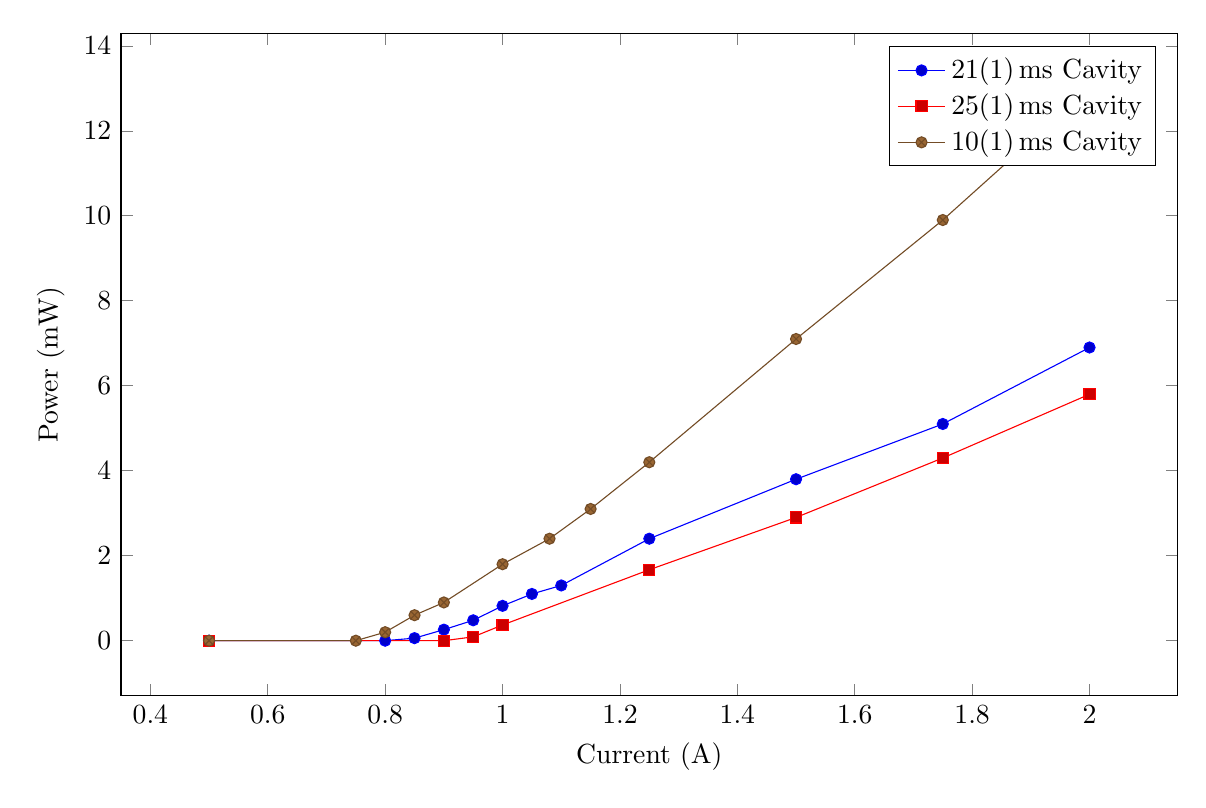
\begin{tikzpicture}
        \begin{axis}[
            xlabel = Current (\si{\ampere}),
            ylabel = Power (\si{\milli\watt}),
            width = 15cm,
            height = 10cm
        ]
            \addplot table {
                2.00	6.9
                1.75	5.1
                1.50	3.8
                1.25	2.4
                1.10	1.3
                1.05	1.1
                1.00	0.82
                0.95	0.48
                0.90	0.26
                0.85	0.06
                0.80	0
                0.50	0
            };
            \addlegendentry{\SI{21 \pm 1}{\milli\second} Cavity}
            \addplot table {
                2.00	5.8
                1.75	4.3
                1.50	2.9
                1.25	1.67
                1.00	0.37
                0.95	0.09
                0.90	0
                0.50	0
            };
            \addlegendentry{\SI{25 \pm 1}{\milli\second} Cavity}
            \addplot table {
                2.00	13
                1.75	9.9
                1.50	7.1
                1.25	4.2
                1.15	3.1
                1.08	2.4
                1.00	1.8
                0.90	0.9
                0.85	0.6
                0.80	0.2
                0.75	0
                0.5	0
            };
            \addlegendentry{\SI{10 \pm 1}{\milli\second} Cavity}
        \end{axis}
    \end{tikzpicture}
    \caption{YAG power verses current for different cavity sizes}
    \label{fig:4.4-power}
\end{figure}

The spectra of the YAG output with and without the \SI{1000}{\nano\metre} pass filter are shown in Figure \ref{fig:4.4-spectra}, with corresponding transmission in Figure \ref{fig:4.4-transmission}. Both were taken with a ND4 filter, with a \SI{1}{\milli\second} integration time, and averaged over 50 readings. There is a clear peak at \SI{1067.5 \pm 0.2}{\nano\metre}. The cavity length was \SI{21 \pm 1}{\milli\metre}.

The average value of the filter transmission in the 1060-\SI{1075}{\nano\metre} range was \SI{0.76 \pm 0.10}{}.

Adjusting the cavity length and taking current-power measurements produces the values in Figure \ref{fig:4.4-power}. Time only allowed for three different cavity lengths to be measured, but one can see much better efficiency with a \SI{10 \pm 1}{\milli\metre} length compared to \SI{20 \pm 1}{\milli\metre} and \SI{25 \pm 1}{\milli\metre} lengths, as well as a lower threshold current.

% TODO: Maybe get values for the slope efficiency?

\subsection{Frequency Doubling}
\begin{figure}
    \centering
    \begin{tikzpicture}
        \begin{axis}[
            xlabel = Wavelength (\si{\nano\metre}),
            ylabel = Counts (a.u.),
            width = 15cm,
            height = 10cm
        ]
            \addplot +[thin, no marks] table [
                skip first n = 17,
                comment chars = >
            ] {spectra/SHG.txt};
        \end{axis}
    \end{tikzpicture}
    \caption{Spectrum of frequency doubled YAG}
    \label{fig:4.5-spectrum}
\end{figure}

Placing the KTP crystal in front of the YAG beam produced a green beam, though it was not visible unless the safety goggles were removed.

Inserting the OD1 filter, as well as an IR absorber, we obtain the spectrum shown in Figure \ref{fig:4.5-spectrum} (\SI{1}{\milli\second} integration time, averaged over 50 readings). One clearly can see three sharp peaks at \SI{532.4 \pm 0.2}{\nano\metre}, \SI{806.3 \pm 0.2}{\nano\metre} and \SI{1067.3 \pm 0.2}{\nano\metre}. Despite the IR absorber, the spectrum is still dominated by the IR components, indicating either the weakness of the green beam, or the poorness of the absorber.

Leaving the spectrometer running (and even observing just by eye), the strength of the \SI{532.4 \pm 0.2}{\nano\metre} component would fluctuate, going from relatively high power (as shown in the spectrum) to almost nothing, and then back, on the order of seconds.

Additionally, if we set the power meter to \SI{532}{\nano\metre} and put the IR absorber in place, we measure about \SI{2.8}{\milli\watt} without the KTP crystal in the cavity, and about \SI{2.0}{\milli\watt} with (regardless of crystal alignment), indicating that all it's reading is the IR, not the green. Given these results, it is clearly fruitless to attempt to measure the current dependence of the frequency doubled beam.

If we place the crystal outside of the cavity, no green light emission was observed.

\subsection{Q-switched Laser Operation}
We were only able to align the laser for Q-switched operation with only a single cavity length: \SI{26 \pm 1}{\milli\metre}.

For this configuration, the pulse widths and period were all very consistent, with pulse width FWHMs of \SI{12.9 \pm 0.2}{\nano\second} and a period of \SI{184 \pm 16}{\micro\second}.

If we placed the KTP crystal outside of the cavity, then we could observe green light emission from it (though safety glasses still had to be removed, like above).

\section{Discussion}
\subsection{Injection Diode Laser Characterisation}
The spectra for before-the-knee (Figure \ref{fig:4.1-spectrum-low}) and after-the-knee (Figure \ref{fig:4.1-spectrum-high}) is pretty much what one would expect for a laser diode.

Before the knee, the light emission is dominated by spontaneous emission, which is characterised by the large linewidth of the emission line. This is mixed together with a small amount of stimulated emission, which increases as current is increased, decreasing the (relative) linewidth, as one can see from the spectra.

After the knee, the emission is now dominated by stimulated emission, so the linewidth is now quite narrow. One might notice that in our measured spectra, the \SI{1.20}{\ampere} spectrum has a wider linewidth than the other three, but this is most likely an artifact of averaging over multiple readings where the laser mode hopped between two adjacent longitudinal modes, seemingly increasing the linewidth. Additionally, our \SI{1.40}{\ampere} spectrum also has a different centre wavelength --- which is also explained by mode hopping, where the measurement was dominated by a different mode than the others.

\subsection{Transmission of the YAG crystal}
Both the \SI{805.3 \pm 0.2}{\nano\metre} and \SI{808.8 \pm 0.2}{\nano\metre} absorption peaks likely correspond to the \({}^4 I_{9/2} \to {}^4 F_{5/2}\) transitions on the neodymium atom (specifically the \SI{804.4}{\nano\metre} and \SI{808.4}{\nano\metre} transitions), which matches with the transition we want.

The absorption at \SI{805.3 \pm 0.2}{\nano\metre} matches almost exactly with the diode laser's output, and would likely contribute a significant amount to the pumping. The bigger (but slightly lower wavelength) absorption peak at \SI{808.8 \pm 0.2}{\nano\metre} probably also contributes to the pumping.

\subsection{Nd:YAG Laser Characteristics}
The emission wavelength of \SI{1067.5 \pm 0.2}{\nano\metre} is slightly lower than the expected \SI{1064}{\nano\metre}. This could either mean the spectrometer was not that well calibrated, or that the energy levels of the neodymium atom has slightly shifted (e.g., due to bonding).

Adjusting the cavity length to shorter lengths seemingly produced a more efficient laser, as can be seen in Figure \ref{fig:4.4-power}. This is most likely due to the fact that our lasing cavity is of the hemispherical type, where decreasing the cavity length produces a larger stable area on the plane mirror's side (where our gain medium is located), and hence allows more of the gain medium to be used.

\subsection{Frequency Doubling}
The \SI{532.4 \pm 0.2}{\nano\metre} peak is pretty much spot-on to the expected emission from the frequency doubler. The signal, however, was very weak compared to the non-doubled signal, which is quite typical of frequency doubling. Placing the crystal outside of the cavity expectedly produced no discernible signal, since the beam intensity is much lower outside of the cavity and hence produces much lower frequency doubled intensities.

Why the power of the frequency doubled signal fluctuated so quickly is unknown, however.

\subsection{Q-switched Laser Operation}
The extra-cavity frequency doubling could be observed this time around, due to the high intensity of the laser pulses, unlike the low intensity of continuous wave operation.

\end{document}